\begin{ZhChapter}

\chapter{BLE Mesh拓樸建立機制設計}

\section{問題分析}

\subsection{BLE Mesh拓樸建立問題}

在原生FruityMesh架構中,節點的建立與連線並未針對資料匯集或匯出端進行特別設計,因此整體網路並無明確的Root節點。其封包傳輸方式主要採用廣播機制,即每當節點產生封包時,會向所有相鄰節點廣播傳送,期望藉由鄰近節點的重傳將封包推進至目的地。雖然此方法具備一定的自我修復能力,但在多節點、大範圍的Mesh網路中,極易導致封包重複傳送與碰撞,進而產生所謂的「廣播風暴」現象,嚴重影響整體網路效能與穩定性。

為了解決此問題,研究中引入DOT(Destination Oriented Transmission)機制\cite{112TIT00392032},將原先的無向廣播傳輸改為目的導向的封包路由方式,透過樹狀拓樸的建立使資料傳輸路徑更具方向性與效率性。然而,導入DOT排程機制的前提之一,是整個BLE Mesh網路需具備清楚的階層結構,而Sink節點(資料匯集端)必須作為整體樹狀拓樸的根節點。唯有如此,封包才能沿著既定的父子節點路徑,自節點有效匯流至Sink節點,達成DOT排程所需的單向、無冗餘傳輸目標。

然而,由於FruityMesh原生設計並非以Sink節點為中心的拓樸為出發點,現有拓樸建立流程尚無法保證Sink節點必然成為根節點。在未進行拓樸控制調整的情況下,可能出現Sink位置偏移、處於樹葉節點甚至中繼節點等非理想情境。因此,若要在FruityMesh架構中有效實作DOT排程機制,勢必需重新設計拓樸建立邏輯,強制指定使Sink節點始終位於拓樸樹的根部,即使在斷線並重新連線的情況下,亦能恢復其根節點角色,確保網路穩定性與傳輸效能。

\subsection{BLE Mesh封包傳輸問題}

在基於FruityMesh的藍牙低功耗網狀網路(BLE Mesh)傳輸機制設計中,\cite{112TIT00392032}研究已針對封包延遲與封包抵達率等品質指標進行優化,並取得初步成效。該研究藉由導入DOT與DOST排程機制,成功改善了大部分的傳輸延遲與資料完整性。然而,即使在優化機制下,網路中仍不時出現封包遺失(掉封包)與重傳現象,顯示目前的傳輸機制尚存在進一步提升的空間。

造成封包掉落與重傳的關鍵因素之一,在於BLE Mesh網路的流量集中特性。由於整體網路皆以Sink節點作為封包的最終目的地,所有資料封包最終皆會匯集至該節點,導致越接近Sink的節點需承擔更多的中繼與轉發任務。這種負載不均的現象將使中樞節點在短時間內接收到大量傳輸要求,導致中樞節點的Sent buffer資源迅速耗盡。一旦緩衝區爆滿,不僅無法即時處理新進封包,還可能造成排程延遲、封包掉落,進而引發重傳機制啟動,進一步加重網路負載。

為有效緩解此類壅塞現象,需從連線參數層級進行調整,特別是針對Connection Event(CE)與Connection Interval(CI)進行優化配置。透過適當調整CI間隔,可有效控制節點可傳輸封包的節奏與頻寬分配,進一步降低高負載節點的壓力,提升整體封包處理效率。結合連線參數調整機制,可以有效改善封包壅塞問題,以提升BLE Mesh網路在多節點、高流量情境下的服務品質(QoS)。

\section{BLE Mesh拓樸建立機制設計}

本論文提出改善FruityMesh的拓樸建立機制,確保Sink節點始終位於整體網路的根節點,並在斷線後能夠自動恢復其角色。此設計為後續的DOT排程機制提供穩定的基礎,如圖\ref{fig: 提出的拓樸建立流程圖}。

\begin{figure*}[htbp]
    \centering
    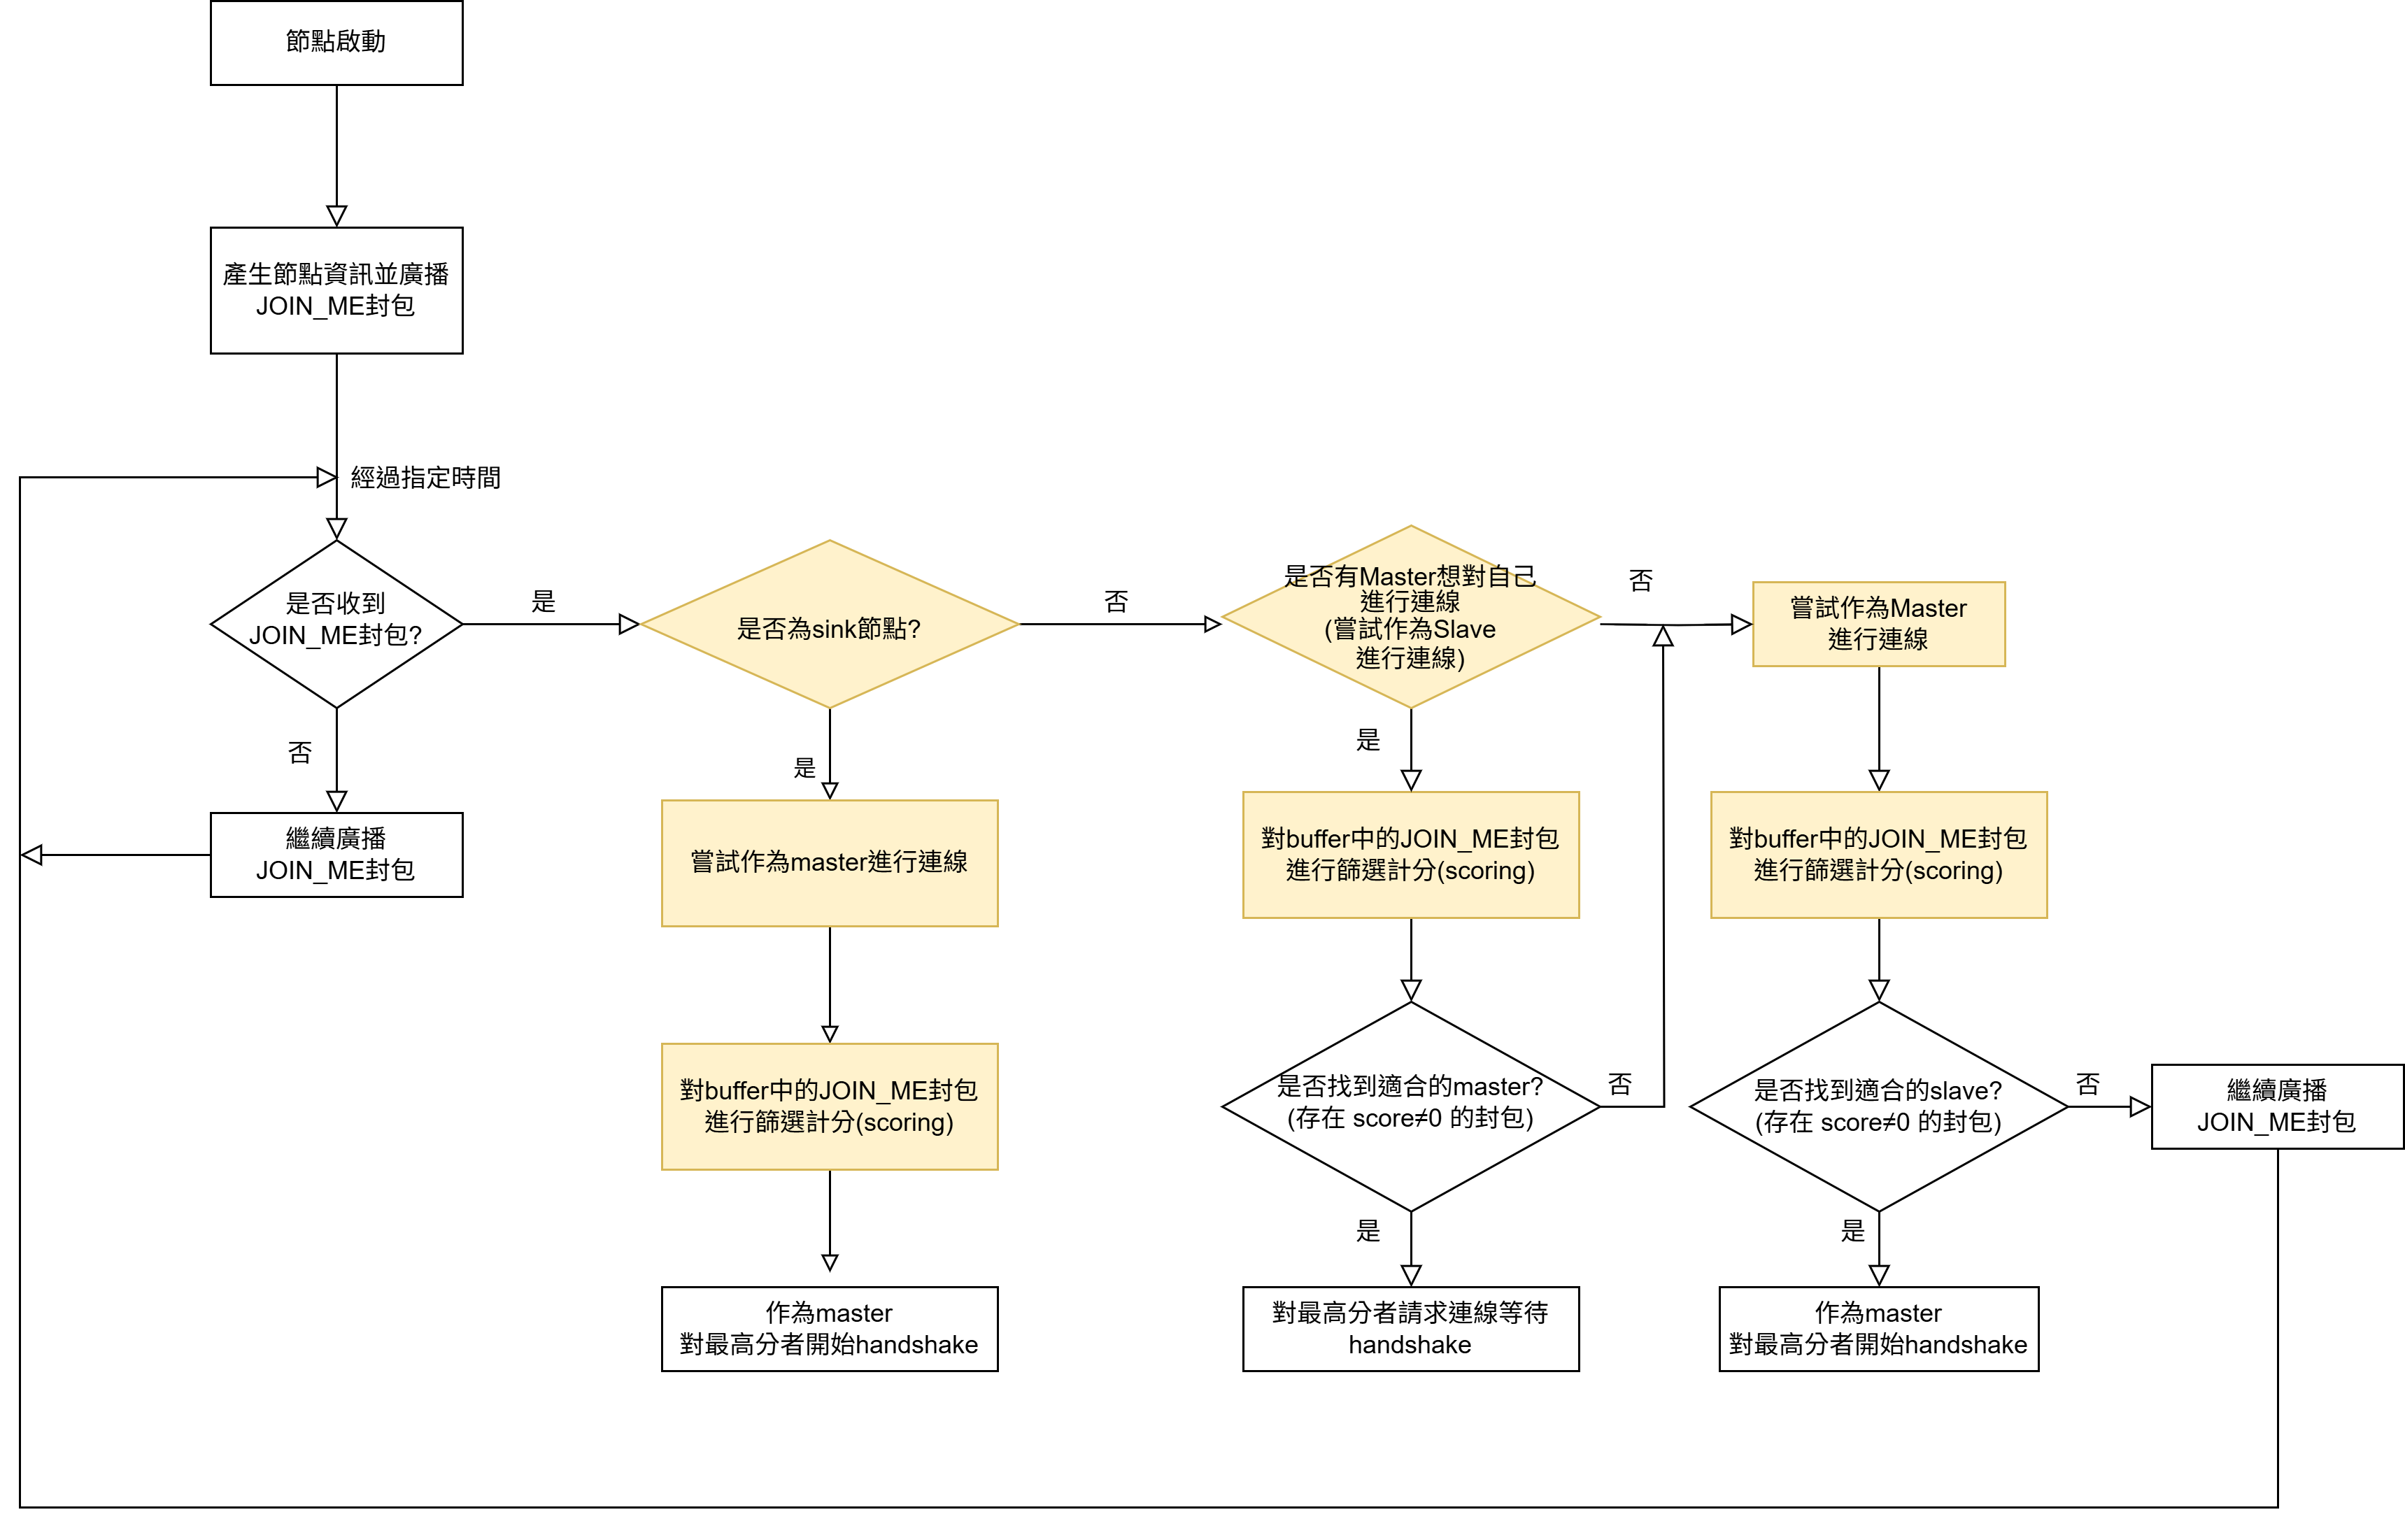
\includegraphics[width = 1\textwidth]{image/build-up_pro2.png}
    \caption{提出的拓樸建立流程圖}
    \label{fig: 提出的拓樸建立流程圖}
\end{figure*}

拓樸建立流程啟動時,每個節點在開機後會廣播包含自身節點資訊的JOIN_ME封包。節點收到其他節點廣播的JOIN_ME封包後,將其儲存於緩衝區中,並根據封包內容進行評分(scoring),以評估對方作為連線對象的適合程度。評分機制可依據鄰近程度、角色可用性(Master/Slave)、RSSI 訊號強度或是否為 Sink 節點等條件進行加權計算。

若節點本身為指定的 Sink 節點,則會主動嘗試作為 Master 發起連線,以確保拓樸的根節點地位。同時,其他非 Sink 節點則會根據收到的 JOIN_ME 封包內容與本地評分結果,決定是否以 Slave 或 Master 身分進行連線。

具體來說,當節點發現有其他節點欲與自己建立連線時(即對方以自己為連線目標進行廣播),會嘗試切換為 Slave 身分接受對方的 Master 連線請求。若尚未與其他節點建立穩定連線,節點會依據緩衝區中評分最高的節點資訊發起連線請求,並進入 handshake 階段以完成連線確認。

透過此機制設計,即使在節點斷線後重新加入網路時,也能根據評分與角色邏輯,回復正確的節點位置與角色,確保整體 BLE Mesh 網路拓樸的一致性與資料流的穩定性。

\end{ZhChapter}